\chapter{\VBFHBB\, Analysis}
\label{c:K}

    After comparing the base constituents of the \VBFHBB\, event between the offline and HLT level and finding them to be similar in behaviour, the specific objects that make up a \VBFHBB\, event can be studied and compared. In this section, the events were required to pass all cuts discussed in Section \ref{es:as} and the designation of the jets as $b_i$, $j_i$ is highlighted in that section. \ref{f:leadingbptvbf}


\section{Cutflow}
\label{k:cutflow}


\section{Specific Jet Feature Distributions}
\label{k:jets}


        \begin{figure}[h]
            \centering
            \begin{minipage}[h]{0.48\linewidth}
                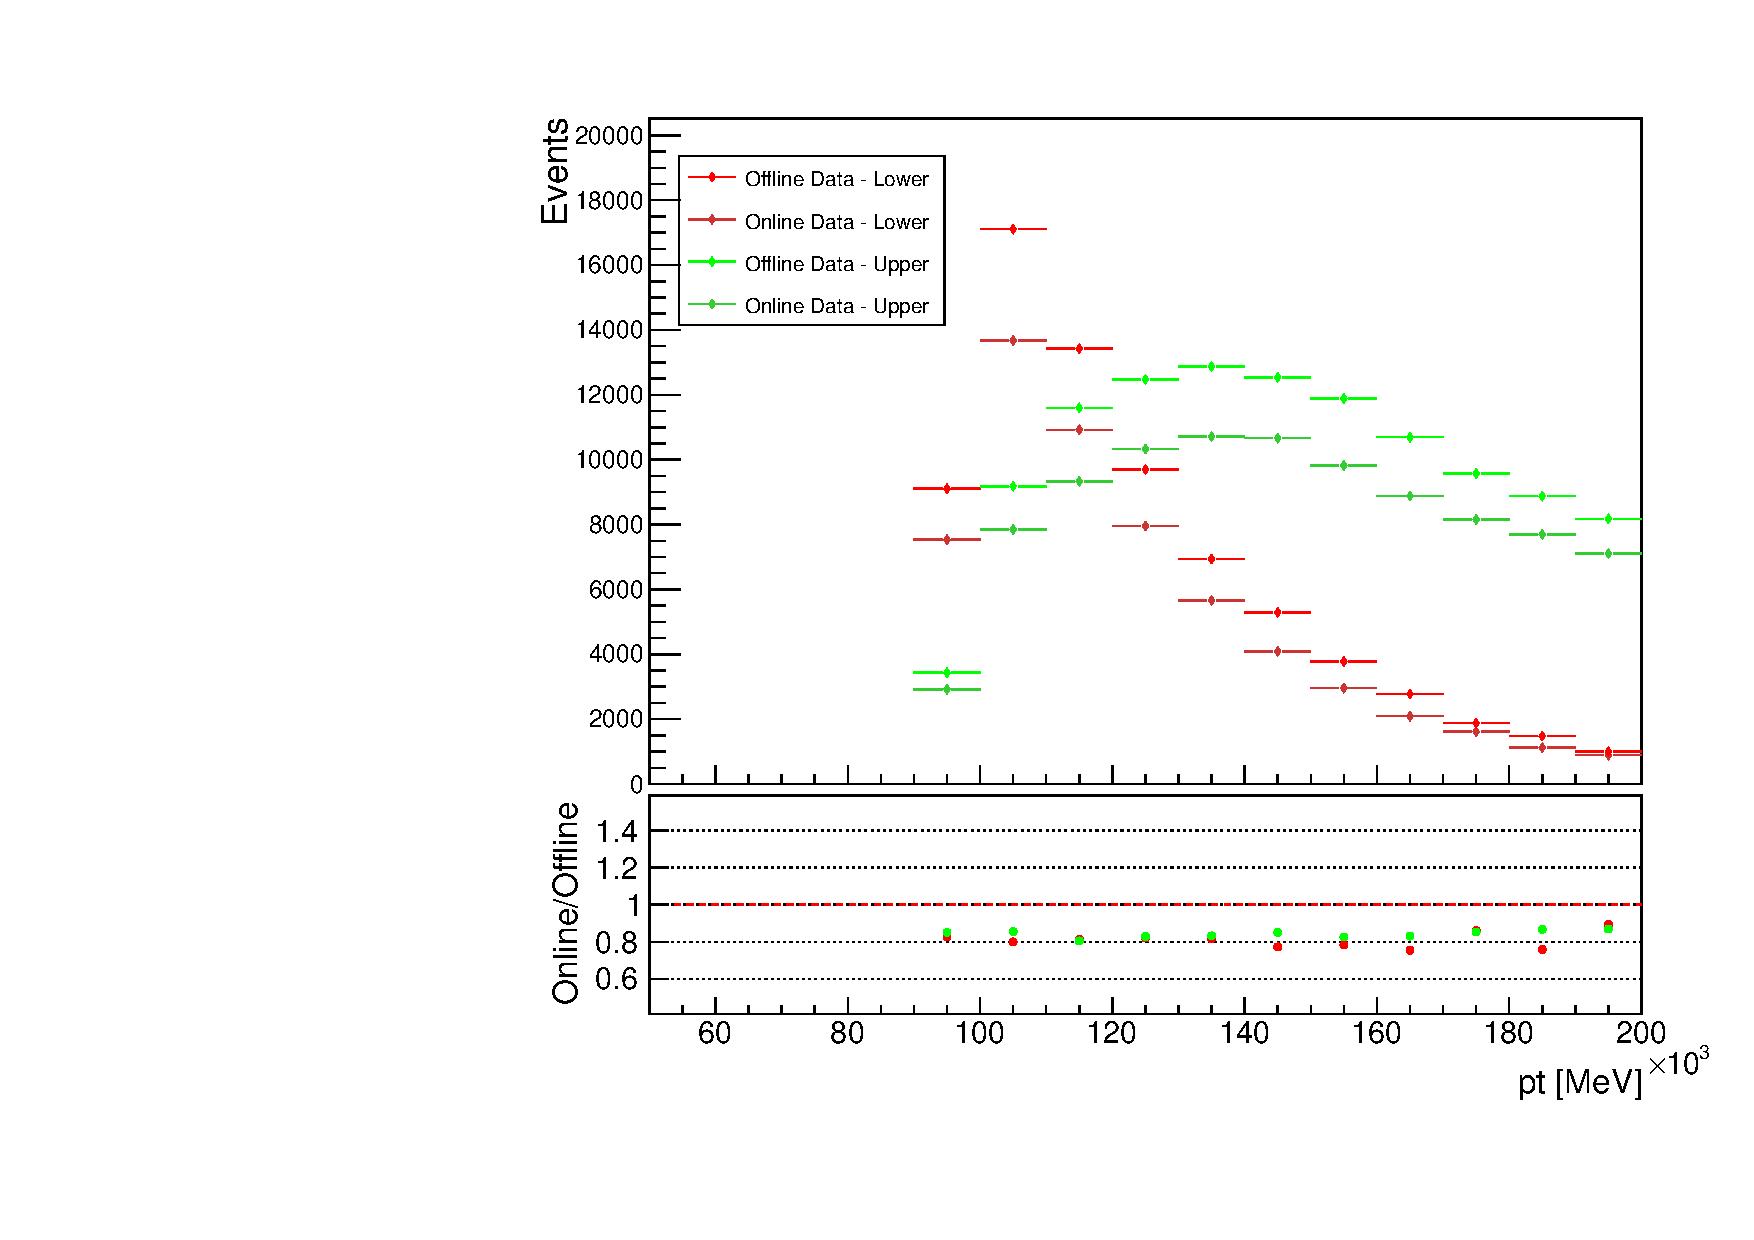
\includegraphics[width=1\linewidth]{pt_bJet1_data_}
            \end{minipage}
            \quad
            \begin{minipage}[h]{0.48\linewidth}
                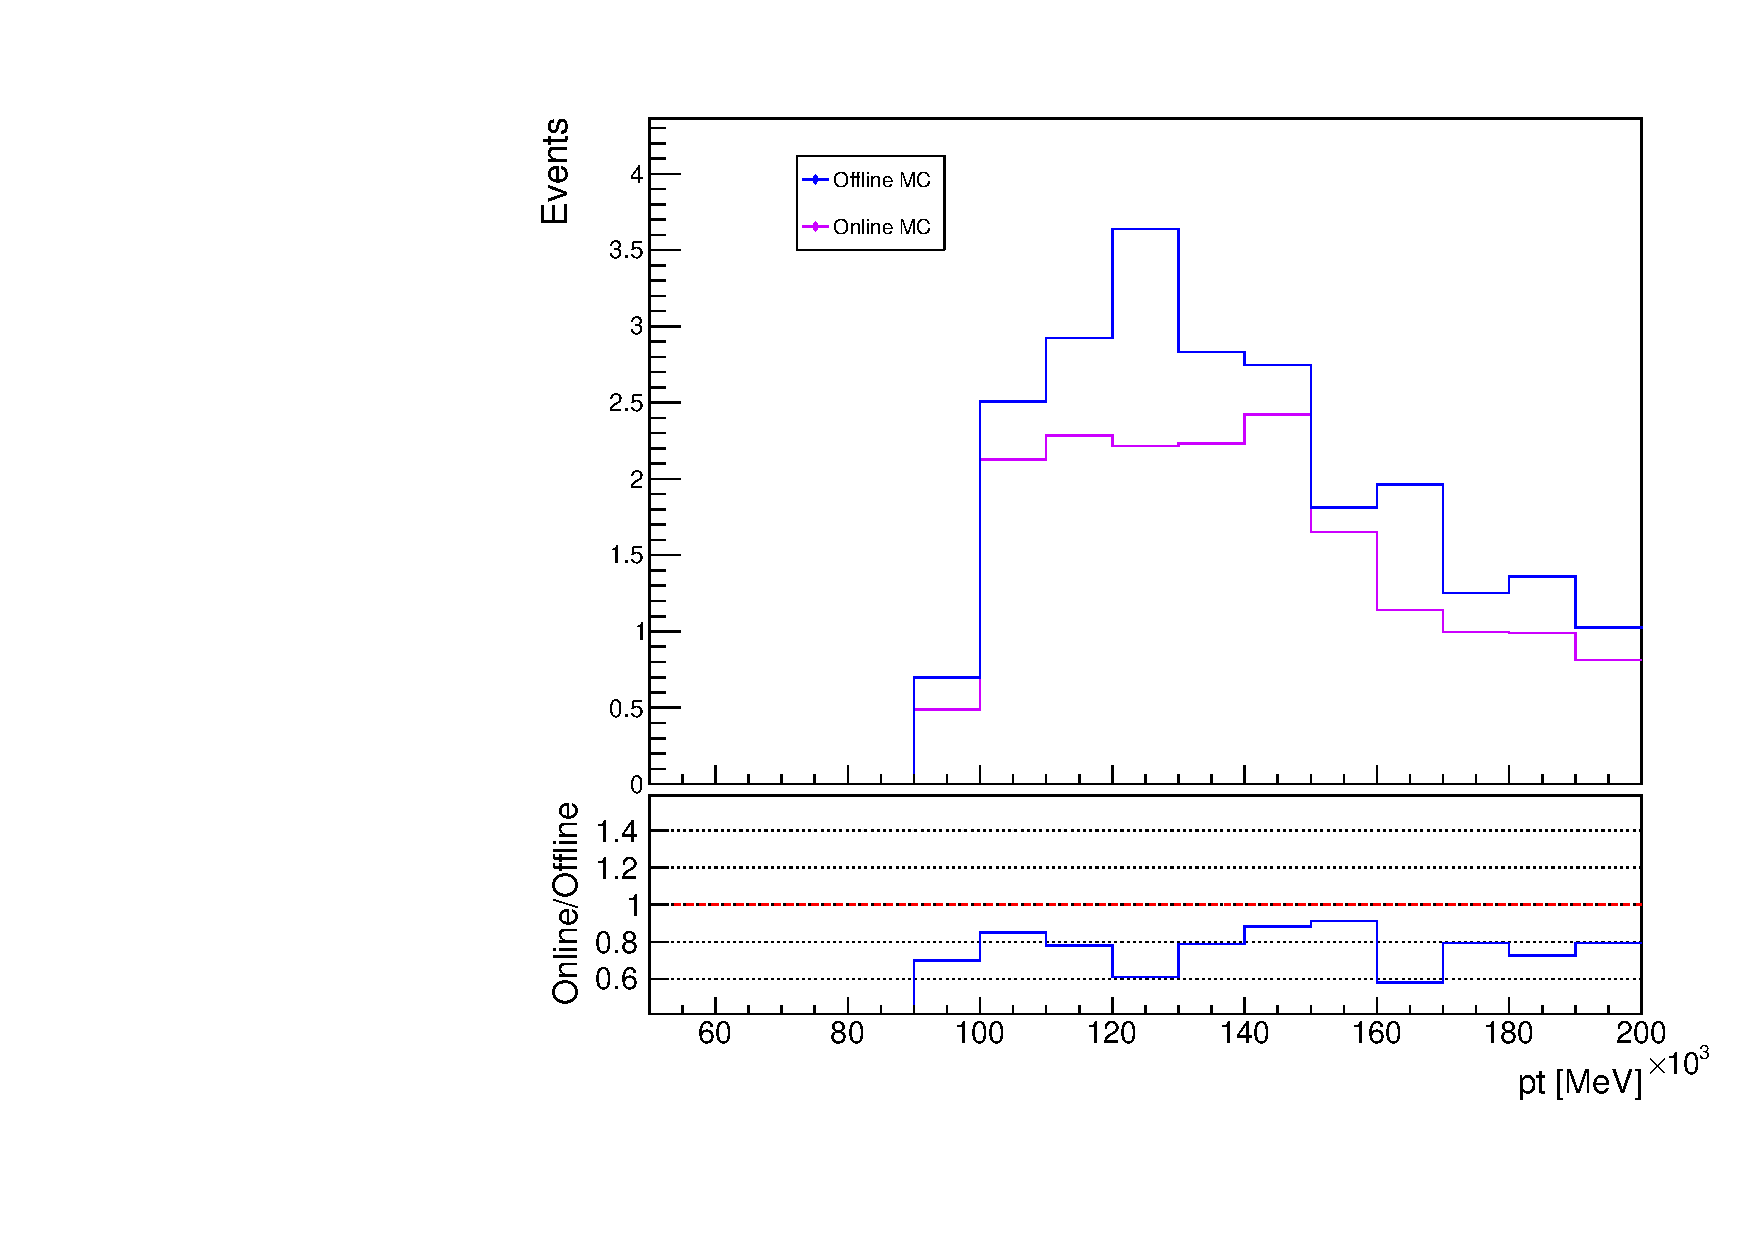
\includegraphics[width=1\linewidth]{pt_bJet1_mc_}
            \end{minipage}
            \caption[\pt distribution of the leading \bjet\ of the \VBFHBB\ event]{\pt distribution of the leading \bjet\ of the \VBFHBB\ event, plotted for both the backgroud data regions in the left panel and Monte-Carlo signal events in the right panel.}
            \label{f:leadingbptvbf}
        \end{figure}
\endinput
